% Drawing 144/07-10 -- folder 144, batch 07, archive page 137 (PDF page 138).
% Transcription: un second diagramme en perspective, même disposition. On y lit : $\mu_{\tau'}\cdot Z^!_{0\rho} = N^{?}_{0\rho}$ (biffé) $\hookrightarrow N^{?}_\rho$, avec au-dessus « $\mu_{\tau'}\cdot Z^!_0$ \ill{} » en partie biffé ; $Z^!_\rho\overset{6}{\hookrightarrow}N_\rho\hookrightarrow\mathcal{M}$ ; $Z^!_{0\rho}\overset{2}{\hookrightarrow}Z^!_\rho\overset{3}{\hookrightarrow}Z_\rho$ ; $\mathcal{M}^!$, $N_\rho$ (indice 6), $\mathcal{M}'$ ; $\mu_{\tau'}\hookrightarrow D_{\tau'}\hookrightarrow D_\rho$ ; $\mathcal{M}'^!_0\overset{2}{\hookrightarrow}\mathcal{M}'^!\overset{6}{\hookrightarrow}\mathcal{M}'$ ; $1\overset{2}{\hookrightarrow}\mu\overset{3}{\hookrightarrow}L_\rho$ ; $\underline\Pi_0\overset{2}{\hookrightarrow}\underline\Pi = \mathfrak{S}^{+!}\overset{6}{\hookrightarrow}\underline{\mathfrak{S}}^+$ ; arêtes verticales et diagonales d'indices 2 et 3.
% Kind: second perspective diagram of inclusions (IV), same layout. Method 2 (schematic redraw from the facsimile). Status: ok.
% Notes: Re-read on a tight crop; same layout as 07-9. Nodes: (top) N^?_rho, Z^!_rho -6-> N_rho, M^! -6-> M; (second row) Z^!_{0 rho} -2-> Z^!_rho -3-> Z_rho; (third) mu_tau' -> D_tau' -> D_rho; (fourth) M'^!_0 -2-> M'^! -6-> M'; (fifth) 1 -2-> mu -3-> L_rho; (bottom) Pi_0 -2-> Pi = S^{+!} -6-> S^+. The vertical and diagonal edges are drawn where they run on the page, with the heads he draws (two where the page has two) and the indices 2, 3, 6 where he wrote them; the arrow from the struck node at the top left to N^?_rho is kept. Labels \small. Strike-outs not drawn: the node N^?_{0 rho} after "mu_tau' . Z^!_{0 rho} =" (crossed out on the page) and the partly struck "mu_tau' . Z^!_0 ..." above it are omitted; the label "mu_tau' . Z^!_{0 rho} =" is kept, as it is not crossed. Still differs from the facsimile: hooks are drawn as plain arrows; the overwritten small labels near M^! (N_rho . i, and an arrow M^! -> N_rho) are not drawn; the index on M'^! -> M' is read 6 (it may be sigma); in the crowded centre, a few short strokes (towards mu from above, from M'^!_0 towards D_tau') are left out, and which nodes some verticals join is a reading. The IV and Z_rho at the top right are headings, not drawn. Redrawn 2026-11-09 (issue 128): to check again. Revised 2026-11-09 after Michel's check (#135): the drawing is right; the index on M'^! -> M' is 6 (not sigma), which is also what the transcription reads, so on this point drawing and transcription agree; ok.
% Coordinates: 1 unit = 1 mm = 1/100 of the crop width (bbox in page fractions: [0.15, 0.53, 0.78, 0.79]).
% Redrawn by Claude (claude-opus-5-5), issue #73, 2026-11-09; not checked by a human; not compiled (no TeX in the session).
% Rights: reproduces part of the work -- behind RENDER_TRANSCRIPTS, never published by itself.
\documentclass[tikz,border=3pt]{standalone}
\usepackage{amsmath,amssymb}
\usetikzlibrary{patterns,arrows.meta}
\tikzset{pencil/.style={black!45}, struck/.style={black!35}, mark/.style={circle,draw,inner sep=1.3pt}, pt/.style={circle,fill,inner sep=0.9pt}, opt/.style={circle,draw,fill=white,inner sep=1.1pt}}
\begin{document}
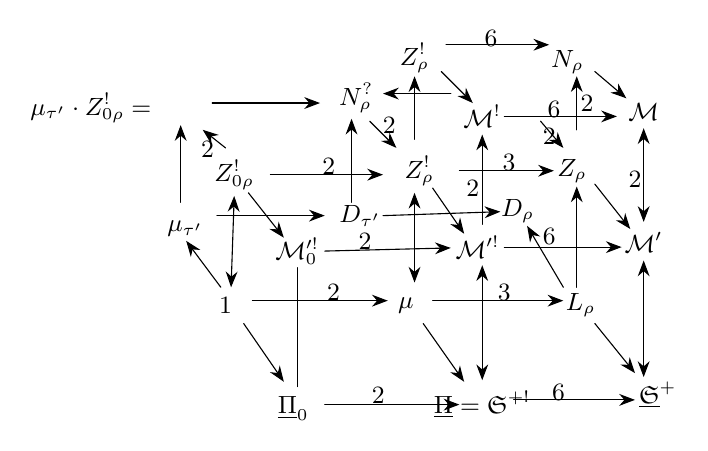
\begin{tikzpicture}[x=1mm,y=1mm,line cap=round,line join=round,font=\scriptsize]
\draw[-{Stealth[length=2mm]}] (23.5,-13.2) -- (37.2,-13.2);
\draw[-{Stealth[length=2mm]}] (19.5,-25.8) -- (19.5,-16);
\draw[-{Stealth[length=2mm]}] (25.2,-18.9) -- (22.3,-16.6);
\draw[-{Stealth[length=2mm]}] (53.8,-12) -- (45.2,-12);
\draw[-{Stealth[length=2mm]}] (53.2,-5.8) -- (66.3,-5.8);
\draw[-{Stealth[length=2mm]}] (52.6,-9.2) -- (56.6,-13.2);
\draw[-{Stealth[length=2mm]}] (72.1,-9.2) -- (76.1,-12.6);
\draw[-{Stealth[length=2mm]}] (69.8,-16.6) -- (69.8,-9.8);
\draw[-{Stealth[length=2mm]}] (60.6,-14.9) -- (74.9,-14.9);
\draw[-{Stealth[length=2mm]}] (49.2,-17.8) -- (49.2,-9.8);
\draw[-{Stealth[length=2mm]}] (41.2,-25.8) -- (41.2,-15.2);
\draw[-{Stealth[length=2mm]}] (43.5,-15.5) -- (46.9,-18.9);
\draw[-{Stealth[length=2mm]}] (30.9,-22.3) -- (45.2,-22.3);
\draw[-{Stealth[length=2mm]}] (54.9,-21.8) -- (66.9,-21.8);
\draw[-{Stealth[length=2mm]}] (51.5,-24) -- (55.5,-29.8);
\draw[{Stealth[length=2mm]}-{Stealth[length=2mm]}] (49.2,-36) -- (49.2,-24.6);
\draw[-{Stealth[length=2mm]}] (69.8,-36.6) -- (69.8,-23.8);
\draw[-{Stealth[length=2mm]}] (72.1,-23.5) -- (76.6,-29.2);
\draw[-{Stealth[length=2mm]}] (65.2,-15.5) -- (68.1,-18.9);
\draw[{Stealth[length=2mm]}-{Stealth[length=2mm]}] (78.3,-16.4) -- (78.3,-28.3);
\draw[-{Stealth[length=2mm]}] (57.8,-28.6) -- (57.8,-17.2);
\draw[-{Stealth[length=2mm]}] (24.1,-27.5) -- (37.8,-27.5);
\draw[-{Stealth[length=2mm]}] (45.2,-27.5) -- (60.1,-27);
\draw[-{Stealth[length=2mm]}] (68.1,-36.6) -- (63.5,-28.8);
\draw[-{Stealth[length=2mm]}] (37.8,-32) -- (53.8,-31.6);
\draw[-{Stealth[length=2mm]}] (60.6,-31.5) -- (75.5,-31.5);
\draw[-{Stealth[length=2mm]}] (28.1,-24.6) -- (32.6,-30.3);
\draw[-{Stealth[length=2mm]}] (24.6,-36.6) -- (20.2,-30.7);
\draw[{Stealth[length=2mm]}-{Stealth[length=2mm]}] (26.3,-25) -- (25.9,-36.6);
\draw (34.3,-34.1) -- (34.3,-49.2);
\draw[-{Stealth[length=2mm]}] (28.6,-38.3) -- (45.8,-38.3);
\draw[-{Stealth[length=2mm]}] (51.5,-38.3) -- (68.1,-38.3);
\draw[-{Stealth[length=2mm]}] (27.5,-41.2) -- (32.6,-48.6);
\draw[-{Stealth[length=2mm]}] (50.3,-41.2) -- (55.5,-48.6);
\draw[-{Stealth[length=2mm]}] (72.1,-41.2) -- (77.2,-47.5);
\draw[{Stealth[length=2mm]}-{Stealth[length=2mm]}] (57.8,-48.4) -- (57.8,-33.8);
\draw[{Stealth[length=2mm]}-{Stealth[length=2mm]}] (78.3,-48) -- (78.3,-33.2);
\draw[-{Stealth[length=2mm]}] (37.8,-51.5) -- (54.9,-51.5);
\draw[-{Stealth[length=2mm]}] (61.8,-50.9) -- (77.2,-50.9);
\node[inner sep=1pt] at (22.9,-19.1) {\small $2$};
\node[inner sep=1pt] at (58.9,-5) {\small $6$};
\node[inner sep=1pt] at (71.1,-13.2) {\small $2$};
\node[inner sep=1pt] at (66.9,-14) {\small $6$};
\node[inner sep=1pt] at (46,-16) {\small $2$};
\node[inner sep=1pt] at (38.3,-21.3) {\small $2$};
\node[inner sep=1pt] at (61.2,-20.7) {\small $3$};
\node[inner sep=1pt] at (66.3,-17.4) {\small $2$};
\node[inner sep=1pt] at (77.2,-22.9) {\small $2$};
\node[inner sep=1pt] at (56.6,-24) {\small $2$};
\node[inner sep=1pt] at (42.9,-30.8) {\small $2$};
\node[inner sep=1pt] at (66.3,-30.2) {\small $6$};
\node[inner sep=1pt] at (38.9,-37.3) {\small $2$};
\node[inner sep=1pt] at (60.6,-37.3) {\small $3$};
\node[inner sep=1pt] at (44.6,-50.4) {\small $2$};
\node[inner sep=1pt] at (67.5,-49.9) {\small $6$};
\node[inner sep=1pt] at (8.1,-13.8) {\small $\mu_{\tau'}\cdot Z^!_{0\rho}=$};
\node[inner sep=1pt] at (41.8,-12.6) {\small $N^?_\rho$};
\node[inner sep=1pt] at (49.2,-7.5) {\small $Z^!_\rho$};
\node[inner sep=1pt] at (68.6,-8) {\small $N_\rho$};
\node[inner sep=1pt] at (57.8,-14.9) {\small $\mathcal{M}^!$};
\node[inner sep=1pt] at (78.3,-14.3) {\small $\mathcal{M}$};
\node[inner sep=1pt] at (26.3,-22.3) {\small $Z^!_{0\rho}$};
\node[inner sep=1pt] at (49.8,-21.8) {\small $Z^!_\rho$};
\node[inner sep=1pt] at (69.2,-21.8) {\small $Z_\rho$};
\node[inner sep=1pt] at (20.1,-29.2) {\small $\mu_{\tau'}$};
\node[inner sep=1pt] at (42.3,-27.5) {\small $D_{\tau'}$};
\node[inner sep=1pt] at (62.3,-26.9) {\small $D_\rho$};
\node[inner sep=1pt] at (34.3,-32) {\small $\mathcal{M}'^!_0$};
\node[inner sep=1pt] at (57.2,-31.5) {\small $\mathcal{M}'^!$};
\node[inner sep=1pt] at (78.3,-30.9) {\small $\mathcal{M}'$};
\node[inner sep=1pt] at (25.2,-38.9) {\small $1$};
\node[inner sep=1pt] at (48.1,-38.9) {\small $\mu$};
\node[inner sep=1pt] at (70.3,-38.9) {\small $L_\rho$};
\node[inner sep=1pt] at (33.8,-52) {\small $\underline{\Pi}_0$};
\node[inner sep=1pt] at (57.8,-51.5) {\small $\underline{\Pi}=\mathfrak{S}^{+!}$};
\node[inner sep=1pt] at (80.1,-50.3) {\small $\underline{\mathfrak{S}}^+$};
\end{tikzpicture}
\end{document}
